\section{Introducción}

\subsection{1.1. Motivación y relevancia}

Resulta particularmente llamativo cómo la cámara de combustión, ese componente discretamente alojado en el corazón de un turbofan, determina en gran medida el futuro de la aviación comercial. Con el tráfico aéreo proyectado para duplicarse en las próximas dos décadas, la presión por reducir el impacto ambiental choca frontalmente contra las demandas de confiabilidad y eficiencia económica. 

Aunque los diseños convencionales han cumplido su rol durante décadas, estudios numéricos recientes como el de Moreno et al. revelan que los combustores anulares ofrecen distribuciones térmicas más uniformes y un potencial tangible para integrar combustibles sostenibles de aviación (SAF). 

Particularmente en motores de la familia CFM56, las simulaciones CFD demuestran mejoras en la mezcla y reducción de puntos calientes que tradicionalmente comprometen la durabilidad de los materiales. 

\begin{table}[h]
\centering
\caption{Requisitos regulatorios ICAO para emisiones en motores de aviación (selección CAEP/8-CAEP/11)}
\label{tab:icao_requirements}
\begin{tabular}{lcc}
\hline
Parámetro & Límite CAEP & Tendencia actual \\
\hline
NOx (g/kN) & 40-60 (según thrust) & Reducciones >30\% necesarias al 2035 \\
CO & 20-80 & Enfoque en idle \\
HC & 4-20 & Casi eliminado en diseños modernos \\
\hline
\end{tabular}
\end{table}

La Tabla 1 resume la evolución de los estándares ICAO, que imponen reducciones drásticas en óxidos de nitrógeno y partículas. Cumplirlos sin sacrificar el desempeño específico del combustible se ha convertido en el principal cuello de botella para los fabricantes.

\subsection{1.2. Evolución histórica de los combustores}

Lejos de ser un asunto resuelto, la transición entre arquitecturas refleja compromisos constantes entre manufacturabilidad, mantenimiento y rendimiento aerotérmico. Los combustores tipo can (tubulares) dominaron las primeras etapas de la propulsión a chorro por su simplicidad de prueba y reparación. Posteriormente, los can-anulares ofrecieron un balance práctico, permitiendo acceso individual a las llamas mientras mantenían una envolvente anular.

Resulta revelador observar cómo, ya en proyectos como el TechCLEAN de JAXA, Makida y colaboradores demostraron que los combustores anulares completos podían alcanzar reducciones de NOx por debajo del 40\% del estándar CAEP/4 bajo condiciones reales de operación, manteniendo al mismo tiempo bajos niveles de CO e hidrocarburos no quemados. 

Estos experimentos con full annular combustor marcaron un punto de inflexión, al validar que la uniformidad circunferencial y el mejor aprovechamiento del aire de dilución no eran solo promesas teóricas, sino ventajas alcanzables en bancos de prueba a presión y temperatura representativas.

\subsection{1.3. Objetivos de investigación y estructura del artículo}

Uno de los desafíos persistentes al analizar estas arquitecturas radica en la escasez de comparaciones directas, actualizadas y cuantitativas que integren simultáneamente desempeño termodinámico y sostenibilidad bajo condiciones operativas modernas. 

Aunque análisis unidimensionales como el propuesto por Jeong y Ahn para double annular combustors han aportado valiosas herramientas para estimar emisiones, tienden a simplificar excesivamente las interacciones tridimensionales de flujo y mezcla que resultan críticas en entornos de alto bypass ratio. 

El presente trabajo busca llenar esta brecha mediante un análisis comparativo sistemático entre sistemas anulares y can-anulares, evaluando métricas de eficiencia de combustión, perfiles de temperatura, estabilidad de llama y emisiones específicas (NOx, CO, soot) bajo un conjunto consistente de condiciones de vuelo.

\begin{figure}[h]
\centering
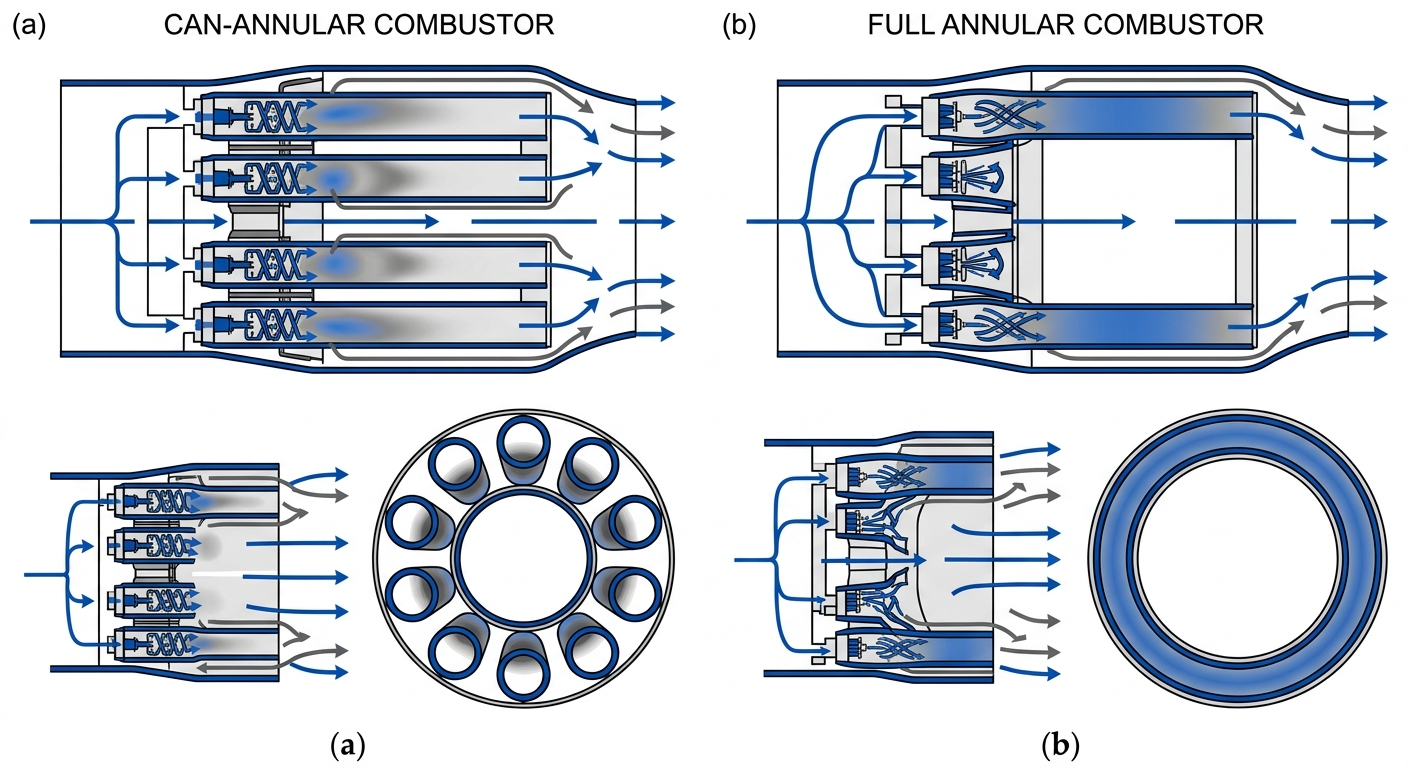
\includegraphics[width=\linewidth]{fig1.png}
\caption{Esquemas comparativos de arquitecturas de combustión: (a) can-anular y (b) anular completo, destacando patrones de inyección de combustible y flujo de aire secundario.}
\label{fig:esquemas_comparativos}
\end{figure}

El artículo se organiza de la siguiente manera: la Sección 2 revisa el estado del arte, la Sección 3 detalla las arquitecturas, mientras que las Secciones 4 a 6 presentan la metodología, resultados de desempeño y evaluación de sostenibilidad. Finalmente, se discuten las implicaciones de diseño y se proponen líneas de investigación futuras.